\chapter{绘制杯立体图}\label{chap:bei}

盛夏,太阳无情的炙烤着大地,树上的知了有气无力的鸣叫着,热浪袭卷着整个城市,人们大多都呆家中或有空调的地方以躲避酷热。秦奋前几日收到了重点高中的取通知书,兴奋过后生活又归于平淡。没有学习压力的他每天除了看电视、上网之外便无事可做。没过几日,好学地他便寻思着找到点来什么事来做或者学点什么。正琢磨着,秦奋的爸爸下班回家了,他灵光一闪:爸爸是高级工程师,他的AutoCAD用得很好,我为什么不跟他学学用AutoCAD绘图,一来可以消磨无聊的生活,二来也可以学项本事,何乐而不为呢!

秦奋立刻去冲了一杯热茶,来到爸爸的书房。爸爸看见儿子端着茶进来,心理很高兴,接过来轻轻地喝了一口,说道:“儿子,谢谢!这可是及时雨啊,你爸的喉咙都快冒烟了!"说完正准备继续看书,见儿子没有走,便问:“你有什么事吗?是不是想玩会儿电脑啊?”

秦奋很认真地说道:“爸,我想跟你学用AutoCAD绘图,平时学习任务重想跟你学,却没有时间。现在离开学还有一个多月的时间,也没有别的学习任务,你看能不能教教我啊?”

爸爸看看认真的秦奋,会心一笑,说:“可以,你想什么时候开始啊?”

秦奋说:“爸,你先休息一下,我去准备一些记录用的纸和笔,然后就开始学习,你看行不?”
爸爸说:“行!”
秦奋回到自己的房间,找出自己用于记录AutoCAD知识的笔记本和笔。而后不紧不慢地回到了他父亲的书房。此时,他父亲已经打开了电脑,准备好了图柢。
爸爸见儿子进来了,说:“我们先从第一张图(图\ref{fig:tiaoyafabei})开始学起,这张图纸中所表示的零件是调压阀中的杯零件,相对来说比较简单,我们今天的目标是学会如何建立它的立体模型。”


\noindent
\begin{figure}[htbp]
\centering
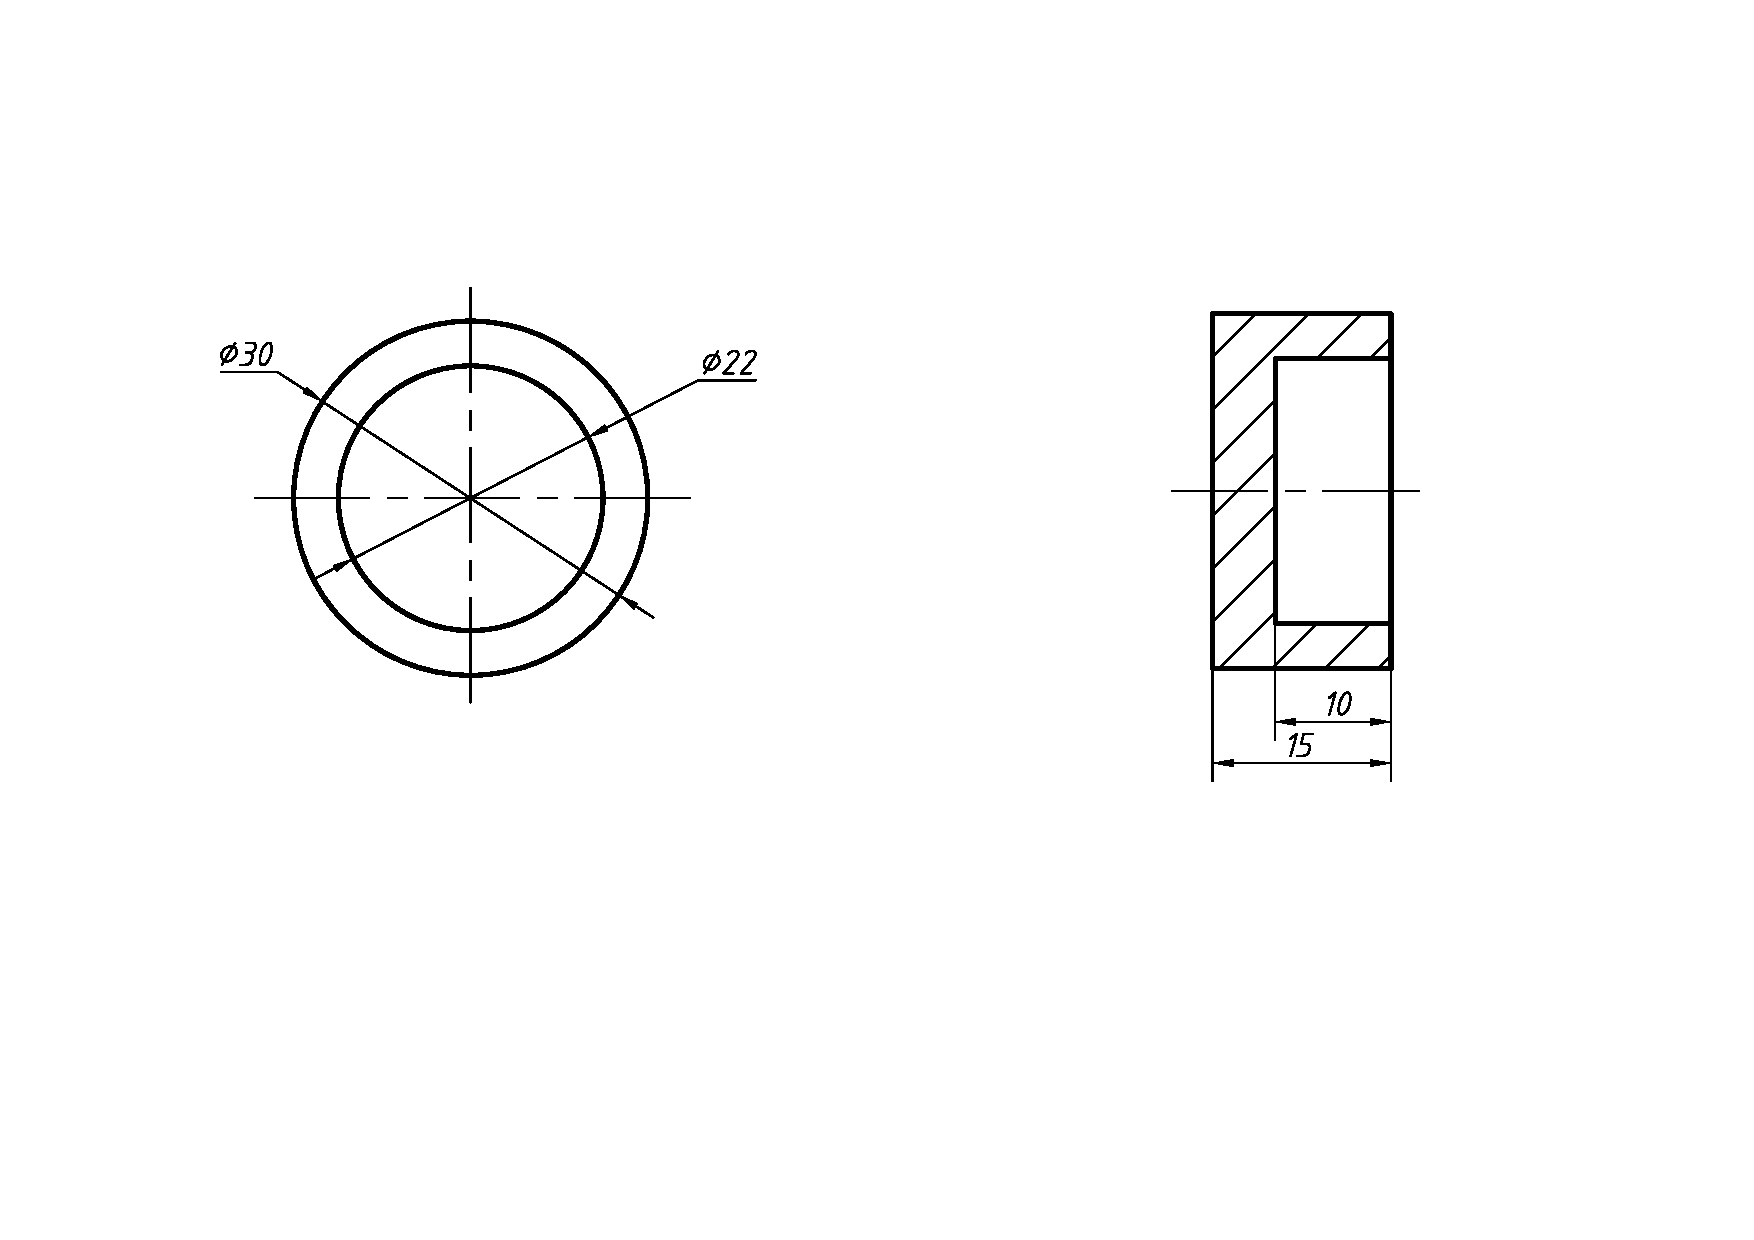
\includegraphics[scale=0.6]{tiaoyafabei.pdf}
\caption{杯零件图}\label{fig:tiaoyafabei}
\end{figure}
\endinput